\begin{figure}
        \centering
        % 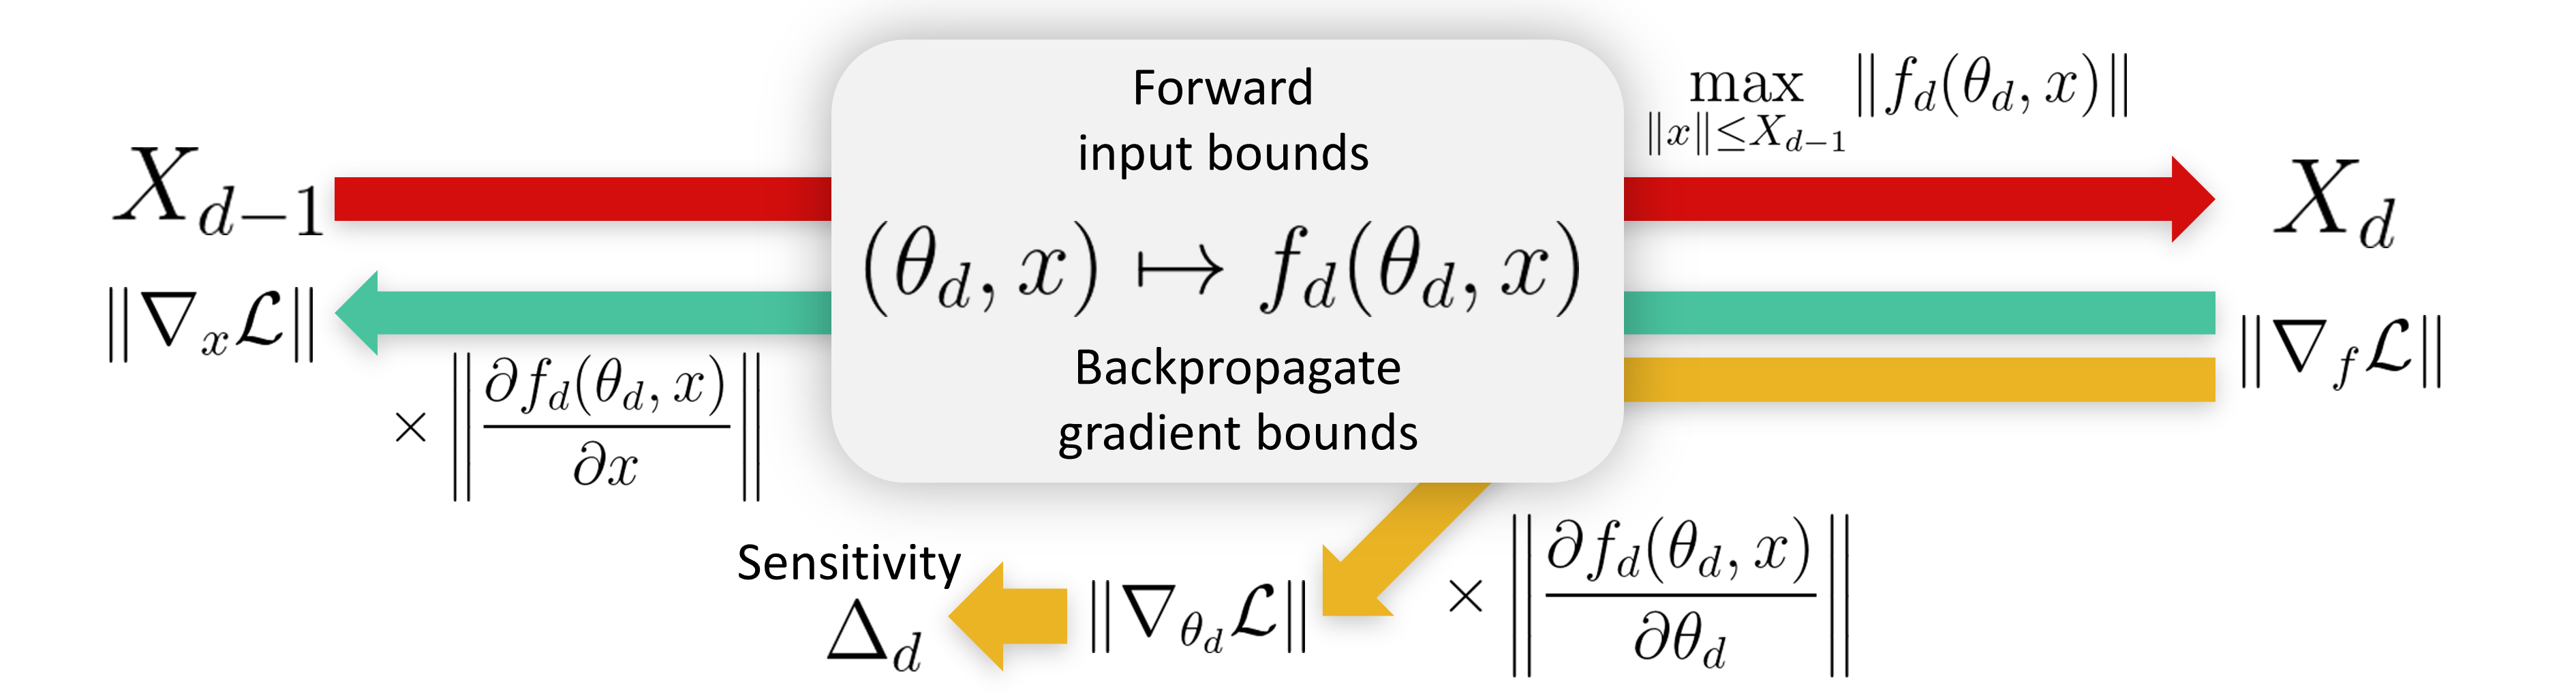
\includegraphics[width=\linewidth]{figures/fig_backprop.png}
        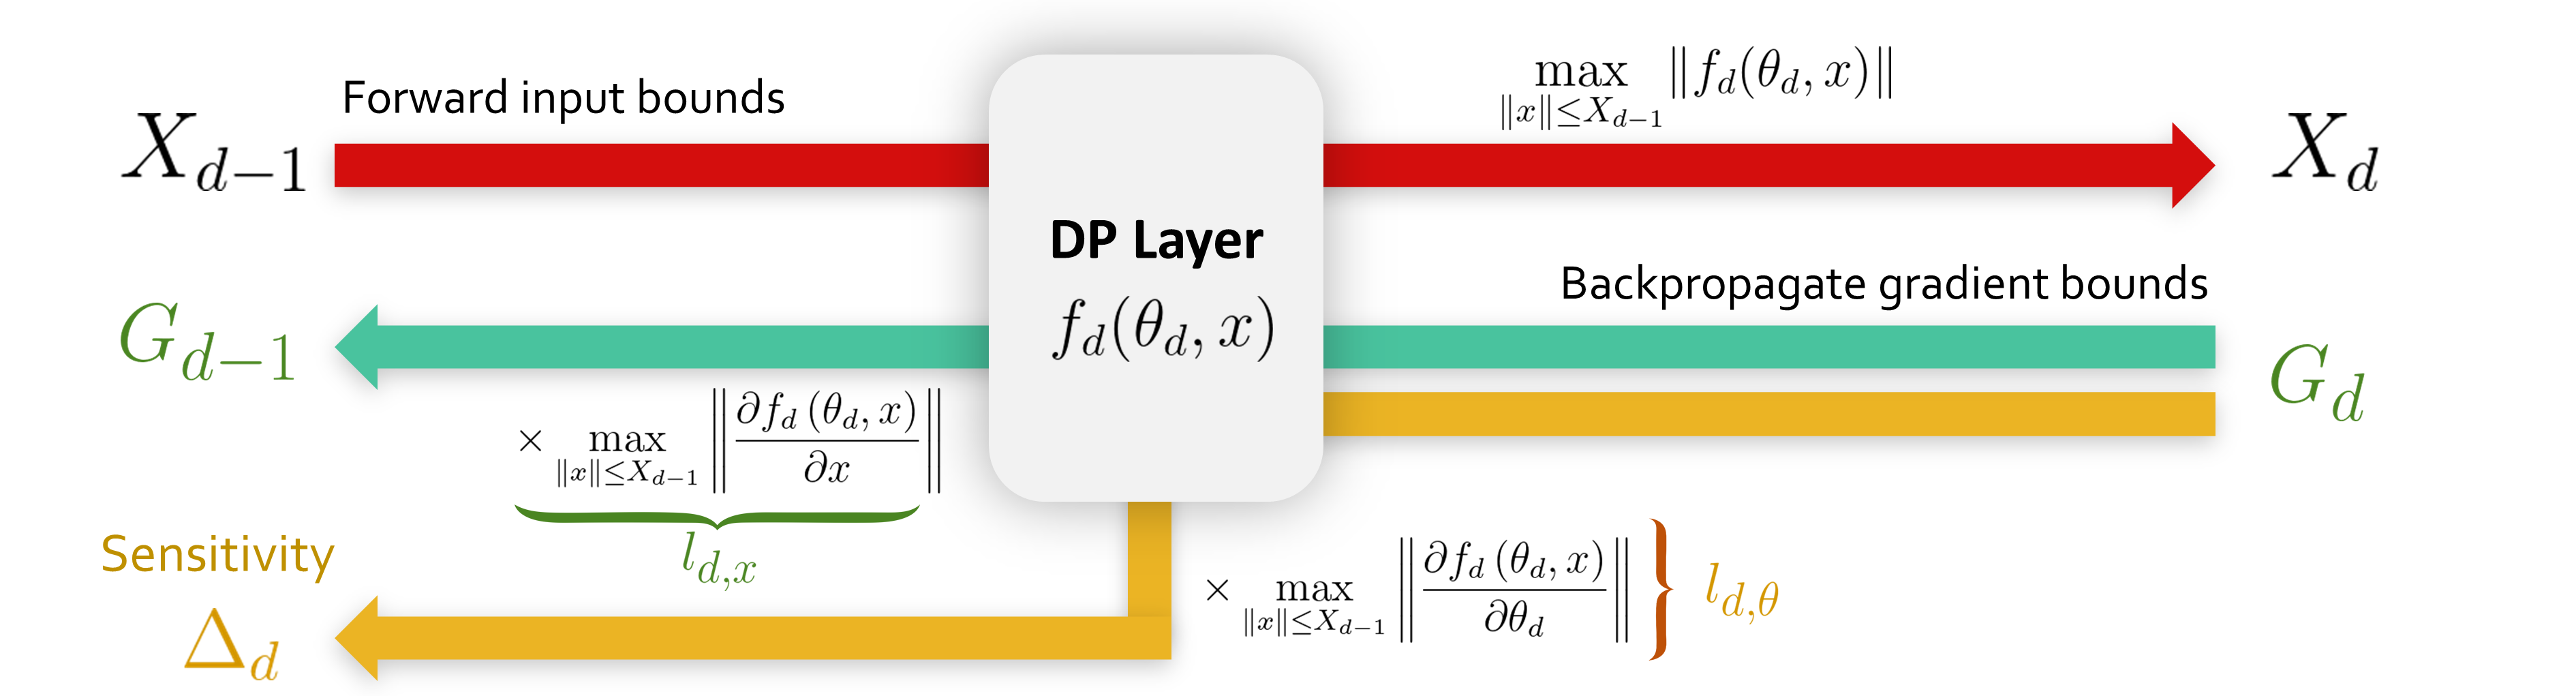
\includegraphics[width=\linewidth]{figures/backprop_v2.png}
        \caption{\textbf{Backpropagation for bounds} (Algorithm~\ref{alg:gnbc}) computes the per-layer sensitivity~$\sntv_d$.}
        \label{fig:backprop}
    \end{figure}
    
    Our framework relies on the computation of the maximum gradient norm of a network w.r.t its parameters to obtain a \textit{per-layer} sensitivity $\Delta_d$. It is based on the recursive formulation of the chain rule involved in backpropagation and requires some natural assumptions that we highlight below.
    
    \begin{requirement}[Lipschitz loss.]\label{req:boundednablal} The loss function $\yhat\mapsto\Loss(\yhat,y)$ must be $L$-Lipschitz with respect to the logits $\yhat$ for all ground truths $y\in\Y$. This is notably the case of Categorical Softmax-Crossentropy.   
    \end{requirement}
    
    The Lipschitz constants of common supervised losses has been computed and reported in the appendix.
    
    \begin{requirement}[Bounded input]\label{req:boundedx}
        There exists $X_0>0$ such that for all $x\in\X$ we have $\|x\|\leq X_0$.  
    \end{requirement}
    
    There exist numerous approaches for the parametrization of Lipschitz networks, such as differentiable re-parametrization (aka ``trivialization'') like~\cite{miyato2018spectral,anil2019sorting}, optimization over matrix manifolds~\citep{absil2008optimization}, direct parametrization~\citep{meunier2022dynamical,wang2023direct}, or projections~\citep{arjovsky2017wasserstein}. We can distinguish two strategies:
    \begin{compactenum}
        \item With a differentiable reparametrization $\Pi:\Reals^p\rightarrow\Theta$ where $\tilde\theta=\Pi(\theta)$: the weights $\tilde\theta$ are used during the forward pass, but the gradients are back-propagated to $\theta$ through $\Pi$. This turns the training into an unconstrained optimization problem on the landscape of $\Loss\circ f\circ \Pi$. \label{enum:reparam}
        \item With a suitable projection operator $\Pi:\Reals^p\rightarrow\Theta$: this is the celebrated Projected Gradient Descent (PGD) algorithm~\citep{bubeck2015convex} applied on the landscape of $\Loss\circ f$. \label{enum:pgd}  
    \end{compactenum}
    Option~\ref{enum:reparam} requires the analysis of the Lipschitz constant of $\Pi$. If $\Theta$ is convex, then $\Pi$ is 1-Lipschitz w.r.t the projection norm, otherwise the Lipschitz constant is generally unknown. For simplicity, option~\ref{enum:pgd} will be the focus of our work.  

    \begin{requirement}[Lipschitz projection]\label{req:pgd}
        The Lipschitz constraints must be enforced with a projection operator $\Pi:\Reals^p\rightarrow\Theta$. This corresponds to Tensorflow \lstinline[basicstyle=\ttfamily, backgroundcolor=\color{gray!20}]{constraints} and Pytorch \lstinline[basicstyle=\ttfamily, backgroundcolor=\color{gray!20}]{hooks}. Projection is a post-processing~\citep{dwork2006calibrating} of private data: it induces no privacy leakage. 
    \end{requirement}

 
To compute the per-layer sensitivities, our framework mimics the backpropagation algorithm, where \textit{Vector-Jacobian} products (VJP) are replaced by \textit{Scalar-Scalar} products of element-wise bounds. For an arbitrary layer $x_d\mapsto f_d(\theta_d,x_d) \defeq y_d$ the operation is sketched below, as a simple consequence of Cauchy-Schwartz inequality:
\begin{align}
    \underbrace{\nabla_{x_d}\Loss\defeq(\nabla_{y_d}\Loss)\Jac{f_d}{x_d}}_{\text{Vector-Jacobian product: backpropagate gradients}} \implies  \underbrace{\|\nabla_{x_d}\Loss\|_2\leq \|\nabla_{y_d}\Loss\|_2\times \textcolor{backwardcolor}{\left\|\Jac{f_d}{x_d}\right\|_2}.}_{\text{Scalar-Scalar product: backpropagate bounds}}
\end{align}
The notation $\|\cdot\|_2$ must be understood as the spectral norm for Jacobian matrices, and the Euclidean norm for gradient vectors. The scalar-scalar product is inexpensive. For Lipschitz layers, the spectral norm of the Jacobian $\|\Jac{f}{x}\|$ is kept constant during training with projection operator $\Pi$. 
The bound of the gradient with respect to the parameters takes a simple form:
\begin{equation}\label{eq:boundparams}
    \|\nabla_{\theta_d}\Loss\|_2\leq\|\nabla_{y_d}\Loss\|_2\times \textcolor{paramcolor}{\left\|\Jac{f_d}{\theta_d}\right\|_2}.
\end{equation}
This term can be analytically bounded, as exposed in the following section.
% Once again the operation is inexpensive since the upper bound $\left\|\Jac{f}{\theta}\right\|_2$ typically depends on the supremum of $\|x_d\|_2$, that can also be analytically bounded, as exposed in the following section.
% The projection operator $\Pi$ ensures that the bounds remain tight throughout training.     

\subsection{Backpropagation for bounds}

    The pseudo-code of \textbf{Clipless DP-SGD} is sketched in Algorithm~\ref{alg:noclipDP-SGDlocal}. The algorithm avoids per-sample clipping by computing a \textit{per-layer} bound on the element-wise gradient norm. The computation of this \textit{per-layer} bound is described by Algorithm~\ref{alg:gnbc} (graphically explained in Figure~\ref{fig:backprop}). Crucially, it requires to compute the spectral norm of the Jacobian of each layer with respect to input and parameters. 

    %\aurelien{je trouve le choix de la notation $X_d$ pas très heureux (ça fait penser à une norme d'input). Peut-être choisir une autre lettre qui évoquerait plutôt les représentations intermédiaires. Ou alors renommer $X$ en $X_0$ pour être consistant.}
    \textbf{Input bound propagation (line~\ref{alg:gnbc:anb}).} We compute $X_d=\textcolor{forwardcolor}{\max_{\|x\|\leq X_{d-1}}\|f_d(x)\|_2}$. For activation functions it depends on their range. For linear layers, it depends on the spectral norm of the operator itself. This quantity can be computed through the SVD or Power Iteration~\citep{trefethen2022numerical,miyato2018spectral}, and constrained during training using projection operator $\Pi$. In particular, it covers the case of convolutions, for which tight bounds are known~\citep{singla2021fantastic}. For affine layers, it additionally depends on the magnitude of the bias~$\|b_d\|$.  


    \begin{remark}[Tighter bounds in literature]\label{remark:forwardbounds}
        Exact estimation of the Lipschitz bound is notoriously an NP-hard problem, as proven by~\citep{virmaux2018lipschitz}. Algorithm~\ref{alg:noclipDP-SGDlocal} can be seen as an extension of their \textit{AutoLip} algorithm to the case of parameters, while their work focused on Lipschitness with respect to the input. Although libraries such as Decomon~\citep{airbus} or \mbox{auto-LiRPA}~\citep{xu2020automatic} provide tighter bounds for $X_d$ via linear relaxations~\citep{singh2019abstract,zhang2018efficient}, our approach is capable of delivering practically tighter bounds than worst-case scenarios thanks to the projection operator $\Pi$, while also being significantly less computationally expensive.  Moreover, hybridizing our method with scalable certification methods can be a path for future extensions.
    \end{remark} 
    
    % \begin{remark}[Tighter bounds in literature.]
    %     Other libraries like Decomon~\cite{airbus} or auto-LiRPA~\cite{xu2020automatic} propose tools based on linear relaxations~\cite{singh2019abstract}\cite{zhang2018efficient} to produce bounds $X_d$ that are typically tighter than our approach~\cite{virmaux2018lipschitz}. Nevertheless, our approach can still provide tighter bounds in practice than worst-case scenarios, thanks to the projection operator~$\Pi$. Furthermore, it does not incur significant computational cost (see section~ \ref{sec:batchspeed}), whereas concurrent methods can spend several hours for medium-sized networks. Finally, bounds that hold over the entire input space $\X$ are typically looser than bounds in the neighborhood of a single example $x$. Our approach is generally compatible with any scalable certification method that can handle this challenge, which opens a path for future extensions.  
    % \end{remark}  
      
    \textbf{Computing maximum gradient norm (line~\ref{alg:gnbc:gnb}).} We now present how to bound the Jacobian $\Jac{f_d(\theta_d,x)}{\theta_d}$. In neural networks, the parameterized layers $f(\theta,x)$ (fully connected, convolutions) are bilinear operators. Hence, we typically obtain bounds of the form:
    \begin{equation} \label{eq:max_grad_norm}
    \textcolor{paramcolor}{\left\|\Jac{f_d(\theta_d,x)}{\theta_d}\right\|_2}\leq K(f_d,\theta_d)\|x\|_2\leq K(f_d,\theta_d)\textcolor{forwardcolor}{X_{d-1}},
    \end{equation}
    where $K(f_d,\theta_d)$ is a constant that depends on the nature of the operator. $X_{d-1}$ is obtained in line~\ref{alg:gnbc:anb} with input bound propagation. Values of $K(f_d,\theta_d)$ for popular layers are reported in the appendix.
    \paragraph{Backpropagate cotangent vector bounds (line~\ref{alg:gnbc:lip}).} Finally, we bound the Jacobian \textcolor{backwardcolor}{$\Jac{f_d(\theta_d,x)}{x}$}. For activation functions, this value can be hard-coded, while for affine layers it is the spectral norm of the linear operator. Like before, this value is enforced by the projection operator~$\Pi$.
    
    \begin{algorithm}%[tb]
    \caption{\textbf{Backpropagation for Bounds}$(f, X)$}
    \label{alg:gnbc}
    \textbf{Input}: Feed-forward architecture $f(\theta,\cdot)=f_{D}(\theta_{D},\cdot)\circ \ldots \circ f_1(\theta_1,\cdot)$\\
    \textbf{Input}: Weights $\theta=(\theta_1,\theta_2,\ldots \theta_{D})$, input bound $X_0$%\\
    \begin{algorithmic}[1] %[1] enables line numbers.
    \For{\textbf{all} layers $1\leq d\leq D$}
        \State $X_d \gets \textcolor{forwardcolor}{\underset{\|x\|\leq X_{d-1}}{\max}\|f_d(\theta_d,x)\|_2}.$ \Comment{Input bounds propagation} \label{alg:gnbc:anb}
    \EndFor
    \State $G\gets L/b.$\Comment{Lipschitz constant of the (averaged) loss for batchsize b} 
    \For{\textbf{all} layers $D\geq d\geq 1$}
        \State $\Delta_d \gets G \textcolor{paramcolor}{\underset{\|x\|\leq X_{d-1}}{\max}\|\Jac{f_d(\theta_d,x)}{\theta_d}\|_2}$. \Comment{Compute sensitivity from gradient norm} \label{alg:gnbc:gnb}
        \State $G\gets G \textcolor{backwardcolor}{\underset{\|x\|\leq X_{d-1}}{\max}\|\Jac{f_d(\theta_d,x)}{x}\|_2} = G \textcolor{backwardcolor}{l_d}$. \Comment{Backpropagate cotangent vector bounds} \label{alg:gnbc:lip}
    \EndFor
    \State \Return sensitivities $\Delta_1,\Delta_2\ldots ,\Delta_{D}$
    \end{algorithmic}
    \end{algorithm}

    \begin{algorithm}%[tb]
    \caption{\textbf{Clipless DP-SGD} with \textbf{per-layer} sensitivity accounting}
    \label{alg:noclipDP-SGDlocal}
    \textbf{Input}: Feed-forward architecture $f(\theta,\cdot)=f_{D}(\theta_{D},\cdot)\circ \ldots \circ f_1(\theta_1,\cdot)$\\
    \textbf{Input}: Initial weights $\theta=(\theta_1,\theta_1,\ldots \theta_D)$, learning rate $\eta$, noise multiplier $\sigma$.%\\
    \begin{algorithmic}[1] %[1] enables line numbers.
    \Repeat
        \State $\Delta_1,\Delta_2\ldots \Delta_{D}\gets $ \textbf{Backpropagation for Bounds}$(f, X)$.
        \State Sample a batch $\mathcal{B}=\{(x_1, y_1), (x_2, y_2), \ldots, (x_b, y_b)\}$.
        \State Compute the averaged gradient for each layer $d$: 
            $g_{d}\defeq \frac{1}{b} \sum_{i=1}^b \nabla_{\theta_{d}} \Loss (f(\theta, x_i),y_i)).$
        \State Sample per-layer noise: $\zeta_d \sim \mathcal{N}(\bm 0,\sigma \Delta_d)$. 
        \State Perform perturbed gradient step:
            $\theta_{d}\gets \theta_{d}-\eta (g_{d} + \zeta_d)$.
        \State Enforce Lipschitz constraint with projection:
            $\theta_{d}\gets \Pi(\theta_{d})$.
        \State Compute new $(\epsilon,\delta)$-DP guarantees with privacy accountant.
    \Until{privacy budget $(\epsilon,\delta)$ has been reached.}
    \end{algorithmic}
    \end{algorithm}

%\label{sec:accountant}
\textbf{Privacy accounting for Clipless DP-SGD.} We keep track of \DP values with a \textit{privacy accountant}~\citep{abadi2016deep}, by composing different mechanisms. For a dataset with $N$ records and a batch size $b$, it relies on two parameters: the sampling ratio~${p=\frac{b}{N}}$ and the ``noise multiplier''~$\sigma$ defined as the ratio between effective noise strength~$\zeta$ and sensitivity~$\Delta$. We propose two strategies to keep track of $(\epsilon,\delta)$ values as the training progresses, based on either the ``per-layer'' sensitivities $\Delta_d$ (composition of Gaussian mechanisms), or by aggregating them into a ``global'' sensitivity $\Delta=\sqrt{\sum_d\Delta_d^2}$ (single isotropic Gaussian mechanism). We rely on the \lstinline[basicstyle=\ttfamily, backgroundcolor=\color{gray!20}]{autodp}\footnote{\url{https://github.com/yuxiangw/autodp} distributed under Apache License 2.0.} library as it uses the R\'enyi Differential Privacy (RDP) adaptive composition theorem~\citep{mironov2017renyi}, that ensures tighter bounds than naive DP composition. Following standard practices of the community~\citep{ponomareva2023dp}, we used \textit{sampling without replacement} at each epoch (by shuffling examples), but we reported $\epsilon$ assuming \textit{Poisson sampling} to benefit from privacy amplification~\citep{balle2018privacy}.  


